\section{Harness Design}
\label{sec:design}

\subsection{One question per layer}

The harness runs three layers, each with a different scientific question and therefore a different design (Table~\ref{tab:layers}). NIH is the in-domain layer: 1,506 studies, a 19-cell grid (clean plus six degradation types at three severities), four reliance conditions, a precision control for the three 4-bit models, and a five-schema ablation on one model. PadChest is the cross-hospital layer: 1,500 studies at stored resolution plus a blank control. Open-i is the report layer: 947 studies, original and blank, scored as prose.

\begin{table}[t]
\centering
\small
\caption{Per-layer design and delivered calls. The 19-cell grid is run only where the synthetic-degradation question is the target; PadChest and Open-i spend their budget on native shift and report generation instead.}
\label{tab:layers}
\begin{tabular}{llrr}
\toprule
Layer & Design & Cells per model & Delivered calls \\
\midrule
NIH & 19-cell shift + 4 reliance + precision + ablation & 28,614 / 6,024 / 6,024 / 15,060 & 240,960 \\
PadChest & native + blank & 3,000 & 21,000 \\
Open-i & report + blank & 1,894 & 13,258 \\
\midrule
\multicolumn{3}{r}{Total (6 models + LLaVA-Med)} & \textbf{275,218} \\
\bottomrule
\end{tabular}
\end{table}

\textbf{Why not one grid everywhere?} A uniform 19-cell grid on all three layers would add 17 cells per image on PadChest and Open-i. At seven models that is $17\times1{,}500\times7=178{,}500$ calls on PadChest and $17\times947\times7=112{,}679$ calls on Open-i: \textbf{291,179 calls} that re-measure the synthetic-degradation question on cohorts whose scientific value is that they did \emph{not} receive a synthetic perturbation. The per-layer design is not a cheaper approximation of the same study; it is a different allocation of the same budget to three different questions.

\textbf{Contract-exempt stages.} LLaVA-Med is run on PadChest and Open-i because its prose contract is the point of the report layer, but its outputs cannot be parsed into the eight-label schema. The harness records these stages as \texttt{contract\_exempt}: they are executed, kept as evidence, and excluded from metrics. The state file therefore distinguishes ``not run'' from ``run and excluded''---a distinction that a results table alone cannot make.

\begin{figure}[t]
\centering
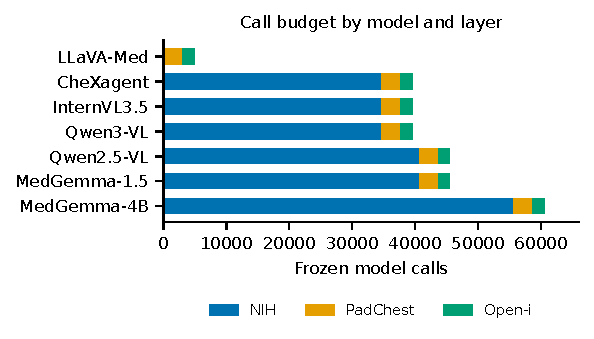
\includegraphics[width=0.82\textwidth]{figures/fig1_calls.pdf}
\caption{Delivered call budget by model and layer. Every bar is recoverable from the JSONL row counts in the frozen matrix; no call is estimated from hours or throughput. LLaVA-Med is contract-exempt and contributes only the two prose layers.}
\label{fig:calls}
\end{figure}

\subsection{Stage ordering and coverage}

Stages run slowest-model-first within each layer, so an interruption is more likely to land on cheap work. The harness also runs a coverage census at the end of every run (CPU only): per file, it counts rows, parse successes, error rows, structured replies, and all-definite replies. A stage that exits zero but whose output has error rows is left incomplete; a stage whose coverage falls below the declared threshold is flagged rather than silently aggregated.
